\documentclass[9pt,twocolumn,twoside]{../../styles/osajnl}
\usepackage{fancyvrb}
\journal{i524} 

\title{Neo4J}

\author[1]{Sowmya Ravi}


\affil[1]{School of Informatics and Computing, Bloomington, IN 47408, U.S.A.}

\affil[*]{Corresponding authors: sowravi@iu.edu.com}

\dates{project-000, \today}

\ociscodes{Cloud, I524}

% replace this with your url in github/gitlab
\doi{\url{https://github.com/cloudmesh/classes/blob/master/docs/source/format/report/report.pdf}}


\begin{abstract}
Neo4J is a graph database designed for fast data access and management. The data is stored in the form of nodes and relationships in Neo4J. The unique approach it takes to store data makes is far more efficient compared to  relational databases when the number of relationships within the data increases. Moreover, it has the ability to store trillions of data entries in a compact manner. Neo4J comes along with Cypher, a highly readable querying language. The paper elaborates the clustering activities used by Neo4j to achieve distributed computing its uses~\cite{www-neo4j-intro}.  

\end{abstract}

\setboolean{displaycopyright}{true}

\begin{document}

\maketitle

\TODO{This review document is provided for you to achieve your
  best. We have listed a number of obvious opportunities for
  improvement. When improving it, please keep this copy untouched and
  instead focus on improving report.tex. The review does not include
  all possible improvement suggestions and for each comment you may
  want to check if it applies elsewhere in the document.}

\TODO{Assessment: Revisions required. Please address the review
  comments below.}

\TODO{Abstract: You need to focus better on what kind of problem and
  data domains Neo4J is suitable for. Saying "... is far more
  efficient compared to relational databases when the number of
  relationships increases" is a bit too general and makes it sound
  like Neo4J and graph databases are a replacement for RDBMSs, which,
  of course, they are not.}

\TODO{Abstract: The last sentence is not grammatical, and it's not
  clear what clustering activities you are referring to. The reference
  is unnecessary and needs to be removed and invoked in the main body
  of the paper.}

\section{Introduction}
Certain problems present in the world cannot be solved by using relational databases. For e.g. a Social \TODO{No reason to capitalize "social"} graph representing a \GE the network of friends in a social networking website. In this case the number of relationships in the data is too extensive and the relational databases perform poorly. \TODO{Please elaborate a little bit on when and why RDBMSs perform poorly to give a better motivation for the existence of Neo4J and graph databases. } Graph data bases on the other hand make the task of storing huge \TE \TODO{"huge" is not descriptive, just use "large". In addition, be specific that it's data that can be modeled as a network of relationships, not data in general.} amounts of data relatively simple and efficient. Neo4J is one such NoSQL, graph database which was developed to be used in the kind of problems mentioned before~\cite{www-neo4j-intro2}. Fig.1 illustrates a simple social network graph. \TODO{This figure is unnecessary. You don't really discuss it, so there is no reason for it to be in the paper.}
\begin{figure}[htbp]
\centering
\fbox{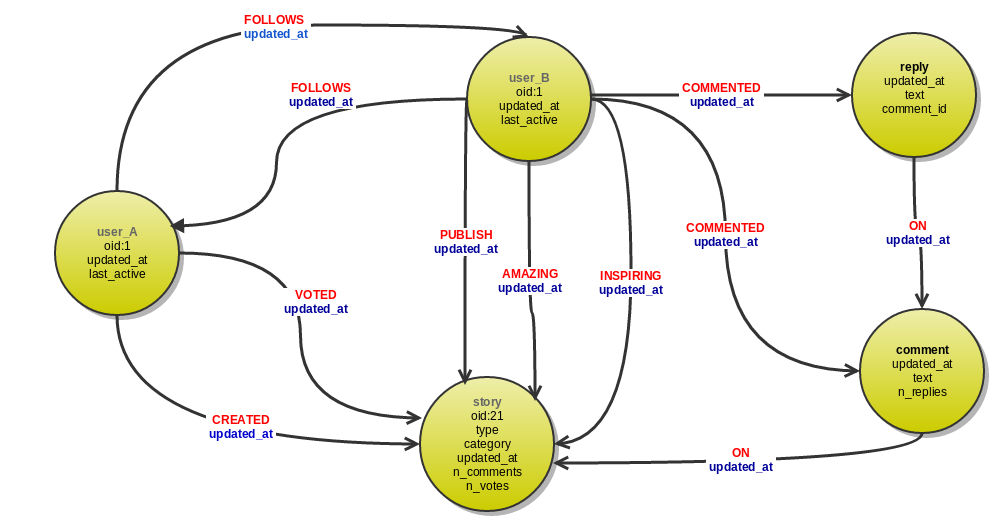
\includegraphics[width=\linewidth]{images/network}}
\caption{A Social Network graph ~\cite{www-graph-img}}
\label{fig:false-color}
\end{figure}


Neo4j is an open source data management software. At its core, Neo4j stores data in the form of nodes and relationships. It is often deployed in a production environment as a fault tolerant cluster of machines. The high scalability and slow traversal times make it far more efficient than the conventional relational databases ~\cite{www-neo4j-intro}. \TODO{Please elaborate. How does slow traversal times make a system more efficient?}

\section{Cypher programing language}
Neo4j uses its own programming language, 
Cypher, for data creation as well as querying. Cypher is capable of doing SQL like actions. In addition, it can specifically perform a powerful query called traversals. Traversal involves moving along a specific set of nodes in the database thereby tracing a path. This allows to leverage the spatial structuring of the data to get valuable information, similar to network 
analysis ~\cite{www-slideshare}. 

\section{Clustering for the enterprise}
This section discusses Neo4js architecture with respect to clustering. \TODO{Why did you choose to focus on clustering? Why is it so important? Please give more detail before you go into the specifics of causal and highly available clustering. Clustering is a term used in many domains, and if someone is not familiar with graph databases, it's unclear how it's used here.} Neo4j uses clustering of machines to achieve high throughput, availability and disaster recovery~\cite{www-neo4j}. Neo4j offers two kind of clustering 
\begin{enumerate}
    \item Causal Clustering
    \item Highly Available clustering
\end{enumerate}

\subsection{Causal Clustering}
The Causal clustering of machines in Neo4j is aimed at providing two important features~\cite{www-neo4j-causal}
\begin{enumerate}
    \item \textbf{Safety}: The core servers of Neo4j ensure fault tolerance.
    \item \textbf{Scalability}: Achieved using Read replicas that make massive scaling possible.
\end{enumerate}
\TODO{The explanation next to "safety" and "scalability" are cryptic and not helpful. What are these core servers? Read replicas? There is no context. You only explain these terms later in the paper.}

The architecture of causal clustering is shown in Fig.2. \TODO{You need to explain what your figures show. Simply referring a reader to a figure is not enough. If you don't elaborate on a figure more, it doesn't need to be in the paper.}
\begin{figure}[htbp]
\centering
\fbox{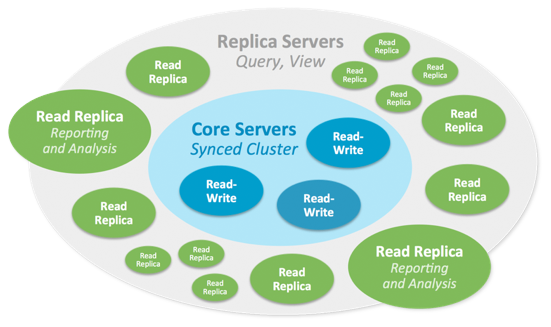
\includegraphics[width=\linewidth]{images/causal-clustering}}
\caption{Architecture of Causal Clustering ~\cite{www-neo4j-causal}}
\label{fig:false-color}
\end{figure}

For operational purposes, the cluster is usually separated into two components: the core servers and the read replicas. 
\subsubsection{Core Servers}
The Core servers are responsible for safe data storage. This is achieved by replicating all incoming queries/transactions using Raft protocol (A log replication protocol)~\cite{www-neo4j-causal}. The protocol ensures the durability of data before committing to the query request. Usually, a transaction is accepted only when a majority of the servers,calculated as $N+1/2$ , have accepted it. This number is directly proportional to the number of core servers $N$. Hence, as the number of core servers grows, the size of majority required for committing to an end user also increases. increases~\TE \cite{www-neo4j-causal}. 

In practice few machines \GE in the core server cluster is enough to provide fault tolerance. This number is calculated using the formula: $N = 2F +1 $ where N is the number of servers required to tolerate F faults~\cite{www-neo4j-causal}. \TODO{Format $N$ and $F$ in math mode every time you invoke them.} When a core server suffers a large number of faults, it is automatically converted to a read-only server for safety purposes. 

\subsubsection{Read replicas}
Read Replicas are Neo4j databases that scale out the incoming queries and procedures. They act like cache memories to the core servers which safeguard the data. Even though the read replicas are full-fledged databases, they are equipped to perform arbitrary read-only activities~\cite{www-neo4j-causal}.

Read Replicas are created asynchronously by core servers through log-shipping~\cite{www-neo4j-causal}. Log shipping occurs when the read replicas poll the core servers for new transactions and the transactions are shipped from the core severs to the read replicas. This polling occurs periodically. Usually, a small number of core servers ship out queries to a relatively large number of read replicas, allowing a large fan out of workload thereby, achieving scalability~\cite{www-neo4j-causal}. The read replicas unlike the core servers do not participate in deciding the cluster topology. 

\subsubsection{Causal Consistency}
In applications, data is generally read from a graph and written to a graph. In order to ensure the causal consistency in the data, the write operation must take into account previous write operations. The Causal Consistency model for distributed computing requires every node in the system to see causally related operations in the same order. This model ensures that the data can be written to cores and the written data be read from read replicas.
Fig.3 illustrates a Causal Cluster with causal consistency

\begin{figure}[htbp]
\centering
\fbox{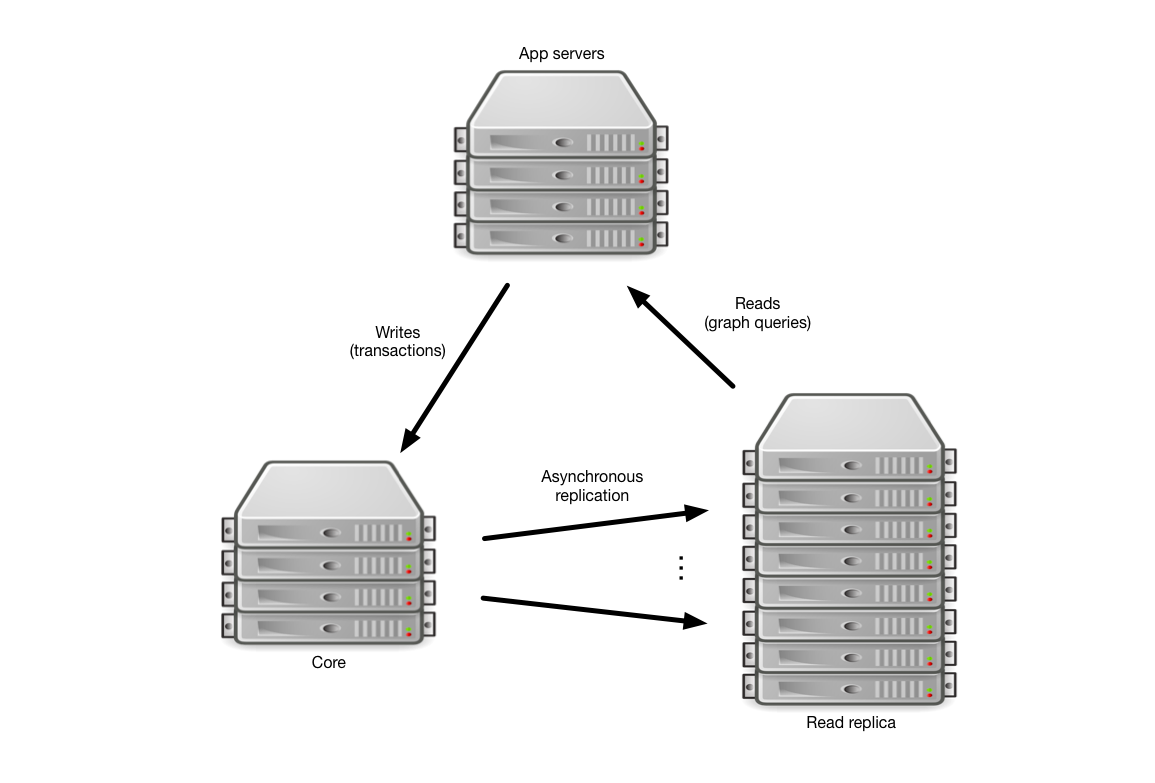
\includegraphics[width=\linewidth]{images/causal-clustering-drivers}}
\caption{Causal Cluster with causal consistency set via Neo4j drivers ~\cite{www-neo4j-causal}}
\label{fig:false-color}
\end{figure}

\section{Highly Available cluster}

\TODO{Please improve the flow of the paper by providing transitions between sections. You start discussing Highly Available Clusters without any relation to the previous section.}

In this type of cluster each instance of the cluster contains full copy of the data in their local database. The cluster can be visualized as containing a single master with multiple slaves in which each instance is connected to every other instance(A 3 member cluster is shown in Fig.4.0) \TODO{You need to refer to a figure by its label. Don't hard code the figure number.}

\begin{figure}[htbp]
\centering
\fbox{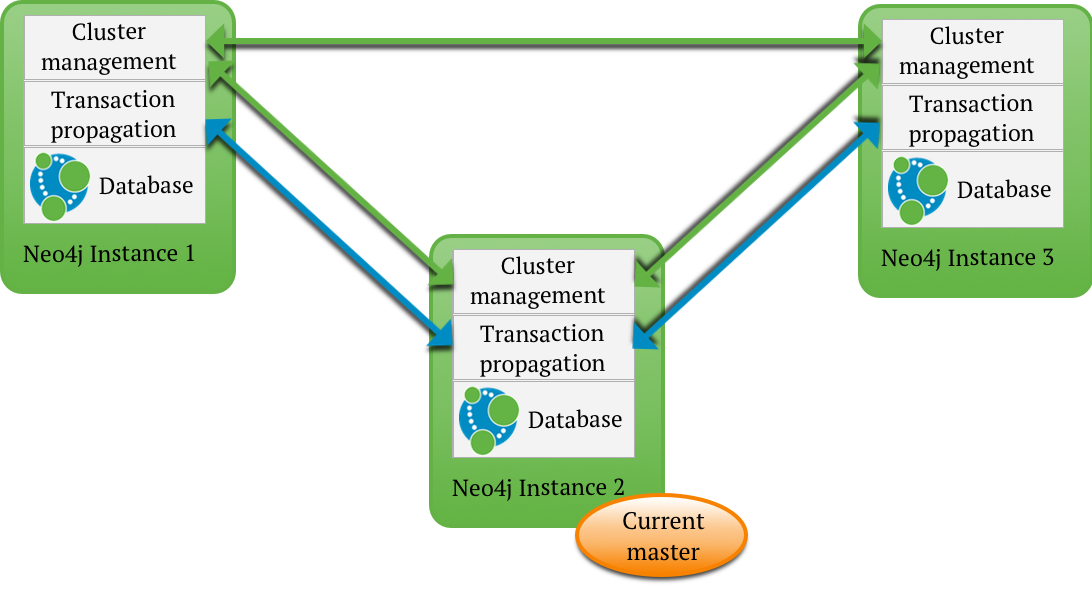
\includegraphics[width=\linewidth]{images/ha-architecture-neo-styled}}
\caption{A Highly Available cluster model~\cite{www-neo4j-ha}}
\label{fig:false-color}
\end{figure}

Also, each instance contains the logic to perform read/write operations and election management~\cite{www-neo4j-ha}. Every slave, excluding the Arbiter instance periodically communicate with the master to keep databases up to date~\cite{www-neo4j-ha}. There is a special slave called the Arbiter explained in the following section.
\subsubsection{Arbiter Instance}
The Arbiter instance is a special slave  that participates in cluster management activities but does not contain any replicated data. It simply contains a Neo4j software running in arbiter mode~\cite{www-neo4j-ha}. 
\subsubsection{Transaction Propagation}
Write Transactions performed directly on the Master will be pushed to slaves once the transaction is successful. When a write transaction is performed on a slave, the slave synchronizes with the Master after each write operation. The write operation on slave is always performed after ensuring that the slave is synchronized with the Master~\cite{www-neo4j-ha}. 

\subsubsection{Failover}
When an instance becomes unavailable, it is marked as temporarily failed by other instances. If the Master fails then, another member in the cluster will be elected as the Master~\cite{www-neo4j-ha}. 

\TODO{This whole section is dropped in the middle of the paper without relation to the other sections. Please, provide better transitions and motivation for why your writing about it.}

\section{Use Cases}
Some of the use case of Neo4j is given below~\cite{www-neo4j-uc}.
\begin{itemize}
    \item Fraud Detection
    \item Graph based search
    \item Network and IT operations
    \item Real-Time Recommendation system
    \item Social Network
    \item Identity and Access Management
\end{itemize}

\TODO{Please don't use so many bullet points. You can simply write a sentence or paragraph that includes the necessary information.}

\subsubsection{Neo4j for Social Network Analysis}
Social Networks are already graphs and several possible use cases for Social Networks are listed below~\cite{www-neo4j-uc2}.
\begin{itemize}
    \item The Friends of Friends recommendation in social networks is one useful use case. The traversal capability makes this task simple and efficient. \TODO{Needs more detail? How does the "traversal capability" makes recommendation easier?}
    \item It can be used to discover previously unknown relationships in massive networks. People get connected through multiple channels. Neo4j may be of great help in studying these relationships \TODO{Incomplete sentence. In addition, what you've described is a type of network analysis that can be performed now matter how the data is organized. How does Neo4J help carry out this analysis?}
    \item Collaboration and Sharing become far more easier in the presence of graph databases. The clustering facility enables data being safe and secure yet highly available. Content visibility increases to a great extent. \TODO{This is not a use case, but a feature of of clustering.}
\end{itemize}

\TODO{This section needs major expansion.}

\section{Conclusion}
Neo4j being an open source, graph based and a highly scalable software, it is suitable for applications that deal with huge amounts of data. \TODO{Not specific enough. It's not simply big data, but data that can be modeled as a netowrk.} Also, Neo4j can be integrated with other tools and software such as Spark, Docker, Elastic Search, MongoDB etc. \TODO{The Conclusion section should summarize what you've covered earlier in the paper. This is the first time you've mentioned integration with these other technologies.} The versatility of Neo4j makes it a great software aid for data scientists trying to analyze relationships and networks in real time as well as in batch. 


% Bibliography

\bibliography{references}
 
\section*{Author Biographies}
\begingroup
\setlength\intextsep{0pt}
\begin{minipage}[t][3.2cm][t]{1.0\columnwidth} % Adjust height [3.2cm] as required for separation of bio photos.
  \begin{wrapfigure}{L}{0.25\columnwidth}
    
\includegraphics[width=0.25\columnwidth]{images/john_smith.eps}
  \end{wrapfigure}
  \noindent
  {\bfseries Sowmya Ravi} pursuing Masters in Data Science from Indiana University. Her research interests include Machine Learning, Data Mining and Big Data Analytics
\end{minipage}

\endgroup

\newpage

\appendix



\end{document}
